\documentclass[type = bachelor]{whu-thesis}
\usepackage{textcomp,mathcomp}
\usepackage{siunitx}
\usepackage{chemfig}
\usepackage{graphicx}

\whusetup
  {
    info               =
      {
        title          = {金刚石氮-空位色心的\\电荷态调控和性质表征},
        title*         = {Modulation of Charge States and Characterization of Properties\\ in Nitrogen-Vacancy Centers of Diamond},
        student-number = {2020302192129},
        school         = {弘毅学堂},
        author         = {邹迪玮},
        author*        = {Diwei Zou},
        subject        = {学科},
        major          = {微电子科学与工程},
        advisor        = {周利 , 副教授;孙启超 , 研究员},
        direction      = {研究方向},
        date           = {2024/5},
        keywords       = {关键词 1 , 关键词 2 , 关键词 3 , 关键词 4 , 一个非常非常,非常非常长——的关键词 5},
        keywords*      = {key word 1 , key word 2 , key word 3 , key word 4 , {and a very very, very very long key word---the key word 5}},
      },
    style              =
      {
        graphics-path  = {{figures/}{data/}},
        list-of-figures,
        list-of-tables,
      },
    element            =
      {
        innovation     = {pages/innovation},
        abstract       = {pages/abstract},
        abstract*      = {pages/enabstract},
        bibliography   = {ref/refs_1}
      }
  }
\begin{document}

% Chapter 1

\chapter{金刚石中的氮-空位色心(NV Center)}

\section{金刚石材料}
金刚石是碳元素的一种常见的同素异形体,在晶体结构上,每一个碳原子被周围的四个碳原子包围并与之形成共价键,从而形成四面体的面心立方结构的晶体。金刚石中的碳原子紧密结合在一起,这样特殊的晶体结构和原子之间稳定的键合方式使得金刚石拥有很多物理和化学上的优异性质,如高硬度、高热导率、高折射率、高抗压强度、高化学稳定性、高电阻率、低热膨胀系数、低摩擦系数、低表面粗糙度、低吸附性等。这些优异的性质使得金刚石在很多领域都有着广泛的应用,如磨料、切割工具、磨料涂层、磁头、光学窗口、高功率激光器件、高频电子器件、生物医学器件等。

金刚石是最坚硬的天然形成的物质,其机械硬度高达 10000 \unit{\kilogram\per\milli\meter\squared},德拜温度高达1860 \unit{\kelvin},它的杨氏模量为1050 \unit{\GPa},有着22 \unit{\watt\per\centi\meter\per\kelvin}的热导率、较低的热展宽系数、较高的击穿电场强度(> 10 \unit{\mega\volt\per\centi\meter}),以及较强的载流子迁移率(对于电子为4500 \unit{\centi\meter\squared\per\volt},对于空穴为3800 \unit{\centi\meter\squared\per\volt})。对于纯净的金刚石而言,其密度为$\rho =$ 3.52 \unit{\g\per\cm},折射率$n =$ 2.39,同时有5.47 \unit{\electronvolt}的较宽带隙,这使其投射光谱范围非常广,从紫外波段(Ultraviolet, UV)到近红外波段(Near Infrared, IR)都可以覆盖到,外观高度透明纯净,拥有极高的透光率 \cite{mildren2013optical, lonvcar2013quantum}。

金刚石在结构上的稳定性使得其化学性质非常的不活跃,因此它几乎不能和大部分化学物质发生反应。所以金刚石有着极低的细胞毒性,使得其在生物、医学领域有着广泛的应用 \cite{schirhagl2014nitrogen,wu2016diamond}。同时,金刚石的化学稳定性也使得其在高温、高压、强腐蚀性环境下有着很好的稳定性,因此金刚石也被广泛应用于高温、高压、强腐蚀性环境下的传感器、探测器等器件中 \cite{umezawa2012high, jayaraman1983diamond}。

由于金刚石晶体的结构非常的整齐和规则,在自然情况下,只有很少一部分的杂质会存在于金刚石晶体中,并参与形成晶格结构。自然界中常见的最主要的金刚石中的杂质是氮和硼元素,因此金刚石可以根据杂质的种类和含量分为不同的类型,主要有两种大类:type \uppercase\expandafter{\romannumeral1}和type \uppercase\expandafter{\romannumeral2},在其中又可以分为四个子类:type \uppercase\expandafter{\romannumeral1}a、type \uppercase\expandafter{\romannumeral1}b、type \uppercase\expandafter{\romannumeral2}a、type \uppercase\expandafter{\romannumeral2}b \cite{breeding2009type}。在这些分类中,type \uppercase\expandafter{\romannumeral1}型的金刚石中主要含有氮元素杂质,type \uppercase\expandafter{\romannumeral1}a型金刚石中的氮元素含量较高,最多有3000 ppm(parts per million,即百万分之一);而type \uppercase\expandafter{\romannumeral1}b型金刚石中的氮元素含量稍低,一般情况下不到500 ppm。由于空气中广泛存在的氮气和土壤中各种各样的氮元素,在自然界中形成的金刚石通常为type \uppercase\expandafter{\romannumeral1}a或者\uppercase\expandafter{\romannumeral1}b。对于type \uppercase\expandafter{\romannumeral2}型的金刚石而言,氮元素的含量远远小于type \uppercase\expandafter{\romannumeral1}型金刚石,通常低于20 ppm。其中,type \uppercase\expandafter{\romannumeral2}b型金刚石中的硼元素杂质含量要高于type \uppercase\expandafter{\romannumeral2}a型。Type \uppercase\expandafter{\romannumeral2}型金刚石的含量极其稀少,而且很少能在自然界中被发现。在科学研究中,type \uppercase\expandafter{\romannumeral2}型金刚石由于其晶体纯净的性质,有着各种各样独特的应用场景。对于科学研究而言,为了保证金刚石样品性质的一致性和实验的可重复性,高纯度和可控掺杂的人造金刚石生长合成技术应运而生 \cite{sumiya1997crystalline, spitsyn1981vapor, gracio2010diamond}。

\subsection{人工合成生长金刚石}
目前主流的人造金刚石样品合成技术主要分为两种,一种是高温高压方法(High Pressure High Temperature,HPHT)和化学气相沉积法(Chemical Vapor Deposition, CVD)。对于HPHT方法而言,其原理主要是模仿天然金刚石在地壳中的形成过程,将碳元素另一种常见的同素异形体石墨的晶体结构在极端的超高温超高压环境下(温度在\SI{1400}{\degreeCelsius}左右,压强在\SI{5.5}{\GPa}左右),通过金属触媒粉的催化作用,转换成具有$sp^3$杂化轨道的金刚石晶体结构 \cite{dossa2023analysis}。HPHT方法使得人类可以在工业上大规模高效率地生产type \uppercase\expandafter{\romannumeral1}型金刚石,但是由于空气中大量的氮气存在,HPHT方法难以生产高纯度低杂质含量的type \uppercase\expandafter{\romannumeral2}型金刚石。由此,为了制备高纯度和可控掺杂的实验级金刚石样品,化学气相沉积的方法逐渐受到科学家们的关注和广泛使用。

CVD方法是一种铜质外延的生长过程,需要在金刚石晶种基面上生长新的金刚石\cite{isberg2002high,isberg2002high}。因此,对于生长出来的晶体,其质量主要取决于晶种的种类和取向,而在非金刚石晶种表面生长会导致生长出有许多单晶金刚石各向同性紧密结合形成的多晶金刚石晶体\cite{mildren2013optical, jahnke2012long}。如果想要形成科学实验中可用的单晶金刚石,就必须用单晶金刚石作为晶种来进行CVD生长。在实际生长的过程中,科学家们通常用{100}取向的晶种衬底来保证尽可能少的生长缺陷\cite{gicquel2001cvd}。

在CVD方法生长金刚石的过程中,除了晶种之外,碳元素源也是比较重要的一个因素。通常情况下,碳元素主要来自于烃类气体,甲烷\chemfig{CH_4}和氢气\chemfig{H_2}的混合气体就是在实验合成的过程中较为理想易得的碳源。对于CVD生长金刚石的过程而言,这些碳源气体需要通过不同的方法来激活,常见的方法有通过热丝(hot filament)或者微波等离子体(microwave plasma),其中微波等离子体气相沉积(Microwave Plasma Chemical Deposition, MPCVD)的方法是生长type \uppercase\expandafter{\romannumeral2}型金刚石最有效的方法\cite{robins1990line, nemanich2014cvd}。在微波等离子体激活后,碳源气体内部形成许多高度反应性的自由基(reactive radicals),活跃的氢自由基(H$\cdot$)有两个重要的功能,一个是终止了已经生长的金刚石表面,从而防止具有$sp^2$杂化轨道的石墨碳原子;其次氢原子可以刻蚀掉已经生成的具有$sp^2$杂化轨道的石墨碳原子,从而在晶种沉底表面上提供悬垂的$sp^3$化学键,使其能够和已经极化的甲基自由基(CH$_3\cdot$)轻松结合,使得单晶金刚石能在沉底表面逐渐生长\cite{denisenko2010surface}。在生长的过程中,各种参数同样十分重要,例如生长腔内压强、温度、气体流速、微波功率等因素决定了生长出来的金刚石的各种性质,使其适用于不同的应用场景。本人于2021年的时候提出了一种n型共掺杂金刚石半导体材料制备的多尺度耦合仿真方法,通过宏观-介观-微观三个尺度的相互耦合,调整MPCVD方法生长金刚石过程中的各种参数,来提高特定用途金刚石的生长合成效率\cite{CN113096749B}。

\subsection{金刚石晶体结构}
金刚石晶体是由每个碳原子和周围四个相邻的碳原子结合,生成四个共价键组成的正四面体结构,其晶格常数为$a_0 = 3.567$ \unit{\angstrom}。金刚石晶体可以看成是两个面心立方晶体的嵌套,其中一个面心立方晶体在三维空间的三个轴上上相对于另一个移动了$\frac{a_0}{4}$,原点从$(0, 0, 0)$移动到了$(\frac{a_0}{4}, \frac{a_0}{4}, \frac{a_0}{4})$。这样的晶体结构使得金刚石非常的坚硬,每一个晶胞中包含着8个碳原子,每一个碳原子的核外电子都呈现$sp^3$杂化轨道结构,和相邻的四个碳原子形成长度为1.44 \unit{\angstrom}的共价键,它的晶体结构见图 \ref{fig: Diamond Lattice}所示。

\begin{figure}[h]
  \centering
  \includegraphics[width=0.9\textwidth]{figures/Chapter 1/Diamond Lattice.png}
  \caption[金刚石及其晶胞结构]{金刚石及其晶胞结构\cite{staudacher2015nuclear}}
  \label{fig: Diamond Lattice}
\end{figure}

然而,在金刚石晶体合成或生长的过程中,晶格缺陷会不可避免的出现,它们会对金刚石的性质产生各种各样的影响,尤其是电子结构产生较大的影响\cite{jelezko2006single, nebel2003electronic}。金刚石晶体中最常见的晶格缺陷是空位(vacancy),这是一种本征晶格缺陷,源于金刚石的中的单个碳原子在其原本的晶格结构上的缺失,每一个孤立的空位可以吸收741 nm的光子,有着高浓度空位的金刚石在一定条件下会呈现蓝绿色的色调,因此金刚石晶体结构中的空位缺陷也被称为色心(color centers),如图 \ref{fig: Color Center}所示\cite{waldermann2007creating, kiflawi2007electron}。

\begin{figure}
  \centering
  \includegraphics[width=0.7\textwidth]{figures/Chapter 1/Color Center.jpg}
  \caption[电子辐照的type \uppercase\expandafter{\romannumeral1}a型金刚石样品显微图片]{电子辐照的type \uppercase\expandafter{\romannumeral1}a型金刚石样品显微图片。浅色区域的空位和氮浓度较低,样品尺寸为\(1\times1\times0.5 \, \mathrm{mm^3}\) \cite{kiflawi2007electron}。}
  \label{fig: Color Center}
\end{figure}

\subsection{金刚石中的色心}
金刚石是一种宽禁带半导体,实验上测得其价带(valence band,VB)和导带(conduction band,CB)之间的带隙宽度大约为5.5 \unit{\eV} \cite{mildren2013optical,cheng2023bandgap,wort2008diamond}。尽管纯净的金刚石呈现无色透明的质地,可以透过的波长范围从UV到IR,但是由于晶格中存在的缺陷或者杂质,使得金刚石体系的带隙之中会出现额外的能级结构,其中的一些能级结构具有活跃的光学性质。因此,这些缺陷结构可以吸收可见光,并在缺陷浓度足够高的时候,使得金刚石材料呈现出特定的颜色,比如高浓度的硼元素会使金刚石呈现蓝色,镍元素相关的缺陷会让金刚石呈现棕色。目前人类已知金刚石中的涉及到光学跃迁性质的荧光缺陷有超过100种,这些缺陷都可以被称为色心\cite{koizumi2008physics,jelezko2006single}。许多的色心都和氮元素杂质有关,因为氮元素是金刚石中最常见的元素,高浓度的氮元素掺杂会使得金刚石呈现黄色的色泽\cite{breeding2020naturally, zaitsev2016spectroscopic}。

金刚石色心种的缺陷能级和电子结构之间的光学跃迁过程可以被人为地进行激光调控,在这个过程中会有不同的激发机理,取决于色心相关的缺陷能级的性质,如图 \ref{fig: Optical Transition}所示。比如,激光的光子可以将缺陷能级的电子激发到导带之中(见图 \ref{fig: Optical Transition}a \uppercase\expandafter{\romannumeral1}所示),或者将电子从夹带激发到缺陷能级见图 \ref{fig: Optical Transition}a \uppercase\expandafter{\romannumeral2所示}。另一种常见的情况是在带隙中有多个缺陷能级的情况,激光可以将电子从一个缺陷能级激发到另一个缺陷能级(见图 \ref{fig: Optical Transition}b所示),这种跃迁的方式相较于电子在缺陷能级和导带(或价带)之间相互跃迁能为高效和可控\cite{gali2011time,gali2012excitation}。在各种各样的色心之中,氮-空位色心(Nitrogen-Vacancy Center)在近些年来被许多科学家所广泛研究,其在532 nm激光的激发下会发出红色的荧光,以此为特征对它的性质进行观测和表征\cite{doherty2013nitrogen}。

\begin{figure}
  \centering
  \includegraphics[width=0.9\textwidth]{figures/Chapter 1/Optical Transition.png}
  \caption[含有缺陷的金刚石晶体的电子能级结构]{含有缺陷的金刚石晶体的电子能级结构。(a)带隙之间的施主和受主能级会使电子发生在价带和缺陷能级(\uppercase\expandafter{\romannumeral1})或缺陷能级和导带(\uppercase\expandafter{\romannumeral2})之间的光学跃迁。(b)电子在施主和受主能级之间的光学跃迁\cite{staudacher2015nuclear}。}
  \label{fig: Optical Transition}
\end{figure}

\section{NV Center的结构和性质}

由于本文主要是围绕金刚石中氮-空位色心的各种性质进行讨论,并结合实验对其进行表征,因此本节将对其结构和性质进行详细的介绍。氮-空位色心不仅仅存在于金刚石中,还可能存在于其他的半导体晶体如碳化硅(SiC)之中,而本文所有的讨论和实验都是基于金刚石中的氮-空位色心,出于方便起见,后文叙述中所有的“NV色心”和“NV Center”都是指金刚石中的氮-空位色心\cite{von2015identification, csore2017characterization}。

\subsection{NV Center的晶体结构}
NV Center是金刚石中最常见的色心之一,其结构如图 \ref{fig: NV Structure}所示,它是由一个氮原子替位原本的碳原子和邻近的一个空位缺陷组成的复合缺陷结构,其晶格结构中的空位缺陷是金刚石晶格中最常见的缺陷,而氮原子是金刚石中最常见的杂质之一,因此NV Center是金刚石中最常见的色心之一。我们定义NV Center的轴向为氮原子和空位中心的连线,也就是晶胞的[111]轴向。氮原子和围绕空位的三个碳原子形成了高度对称的$C_{3v}$对称性结构,这种结构使得NV Center的晶体结构具有很高的对称性(其结构对称性见图 \ref{fig: NV Symmetry}),从而使得NVCenter的电子结构和光学性质具有很高的稳定性。

\begin{figure}
  \centering
  \includegraphics[width=0.9\textwidth]{figures/Chapter 1/NV Structure.png}
  \caption[金刚石中NV Center的结构]{金刚石中NV Center的结构,其中深蓝色的原子为氮原子,橙色的电子自旋标识符处为空位,围绕在NV Center周围的碳原子为深灰色\cite{staudacher2015nuclear}。}
  \label{fig: NV Structure}
\end{figure}

\begin{figure}
  \centering
  \includegraphics[width=1.0\textwidth]{figures/Chapter 1/NV Symmetry.png}
  \caption[金刚石的C$_{3v}$对称性群结构]{金刚石的C$_{3v}$对称性群结构,氮原子和围绕空位(中心半透明标识)的三个碳原子沿着[111]轴旋转对称,同时也沿着每个碳原子分别和空位、氮原子组成的平面镜像对称\cite{doherty2013nitrogen}。}
  \label{fig: NV Symmetry}
\end{figure}

近十几年来,随着半导体的工艺进步和计算机的广泛运用,人们开发了许多强有力的科学计算工具,通过基于密度泛函理论(Density Functional Theory, DFT)第一性原理(First-principles),利用HSE杂化泛函Heyd-Scuseria-Ernzerhof (HSE06)算法可以较为准确地得到NV Center的自旋密度(Spin Density)和带隙中各能级的电荷密度(Charge Density),如图 \ref{fig: Spin and Charge Density}所示,可以看到NV$^-$的自旋密度和带隙中各个缺陷能级的电荷密度都是围绕$C_{3v}$旋转对称\cite{zou2023influence}。

\begin{figure}
  \centering
  \includegraphics[width=1.0\textwidth]{figures/Chapter 1/Spin and Charge Density.png}
  \caption[基态NV$^-$的自旋密度和带隙中各个缺陷能级的电荷密度分布]{基态NV$^-$的自旋密度和带隙中各个缺陷能级的电荷密度分布,其中蓝色的原子为氮原子,棕色的原子为碳原子,视角沿$C_{3v}$轴的[-1 -1 -1]方向,粉红色的区域为自旋密度分布,淡黄色的区域为电荷密度分布,绘图参数isovalue的值设置为0.0078 \unit{e\per\bohr\cubed}\cite{zou2023influence}。}
  \label{fig: Spin and Charge Density}
\end{figure}

由于氮元素是元素周期表上第五主族的元素,所以其外围电子层中有五个价电子,其中三个电子和周围三个碳原子结合形成共价键,剩余两个电子和空位周围的三个碳原子上剩余的一个电子共五个电子形成了中性的NV CenterNV$^0$,因此五个电子形成的自旋系统有一个孤立的电子自旋,所以NV$^0$的电子自旋量子数$S=\frac{1}{2}$。在实验上已经发现的NV Center的两种稳定的电荷态,中性的NV$^0$和带负电的NV$^-$,其中NV$^-$的电子自旋量子数$S=1$ \cite{waldherr2011dark,aslam2013photo,dolde2014nanoscale}。NV Center的电荷态取决于其周围的环境状态,比如附近存在的杂质、缺陷、电场,或者周围的施主、受主能级等,更进一步地,取决于整个金刚石体系的费米能级(Fermi Level,$E_F$)\cite{doherty2013nitrogen}。在金刚石中,NV Center的电荷态可以通过光学方法进行调控,比如通过激光光子的吸收和发射,可以使NV Center的电荷态在NV$^0$和NV$^-$之间进行转换\cite{doi2016pure,siyushev2013optically,shields2015efficient}。通常情况下,NV Center可能并不会处于某种特定单一的状态,而是在两个电荷态之间不断地切换。在NV Center的电荷态切换的过程中,其电子自旋态也会发生变化,这种变化可以通过光学方法进行探测和读出,从而可以对NV Center的电荷态进行探测,这也是本文主要聚焦的问题。

对于NV Center的两种电荷态NV$^0$和NV$^-$而言,我们最主要的区分方式就是其光谱特征的不同,两种电荷态在零声子线处(zero phonon line, ZPL)都有较为强烈的光学跃迁现象。零声子线是指在光谱中的一种特殊峰值或能级跃迁,其特点是在跃迁过程中不伴随着声子(晶格振动)的吸收或发射,此状态下的能级跃迁是非常干净和锐利的,不受热振动的影响,通常情况下接近绝对零度的时候,声子的振动作用极其微弱,晶体的大部分光学跃迁都接近于ZPL的波长。零声子线通常表示了一个非常纯净的能级跃迁,因为它不受晶格振动引起的能级展宽的影响。如图 \ref{fig: NV Spectrum}所示,NV$^-$的零声子线位于637 nm处,而NV$^0$的零声子线位于575 nm处。在室温条件下,由于声子振动不可避免的影响,零声子线总会伴随着较强的声子边带(phonon sidebands, PSB)效应,导致NV Center的光谱出现展宽现象,而不是在ZPL处出现极其尖锐突出的峰值。

\begin{figure}
  \centering
  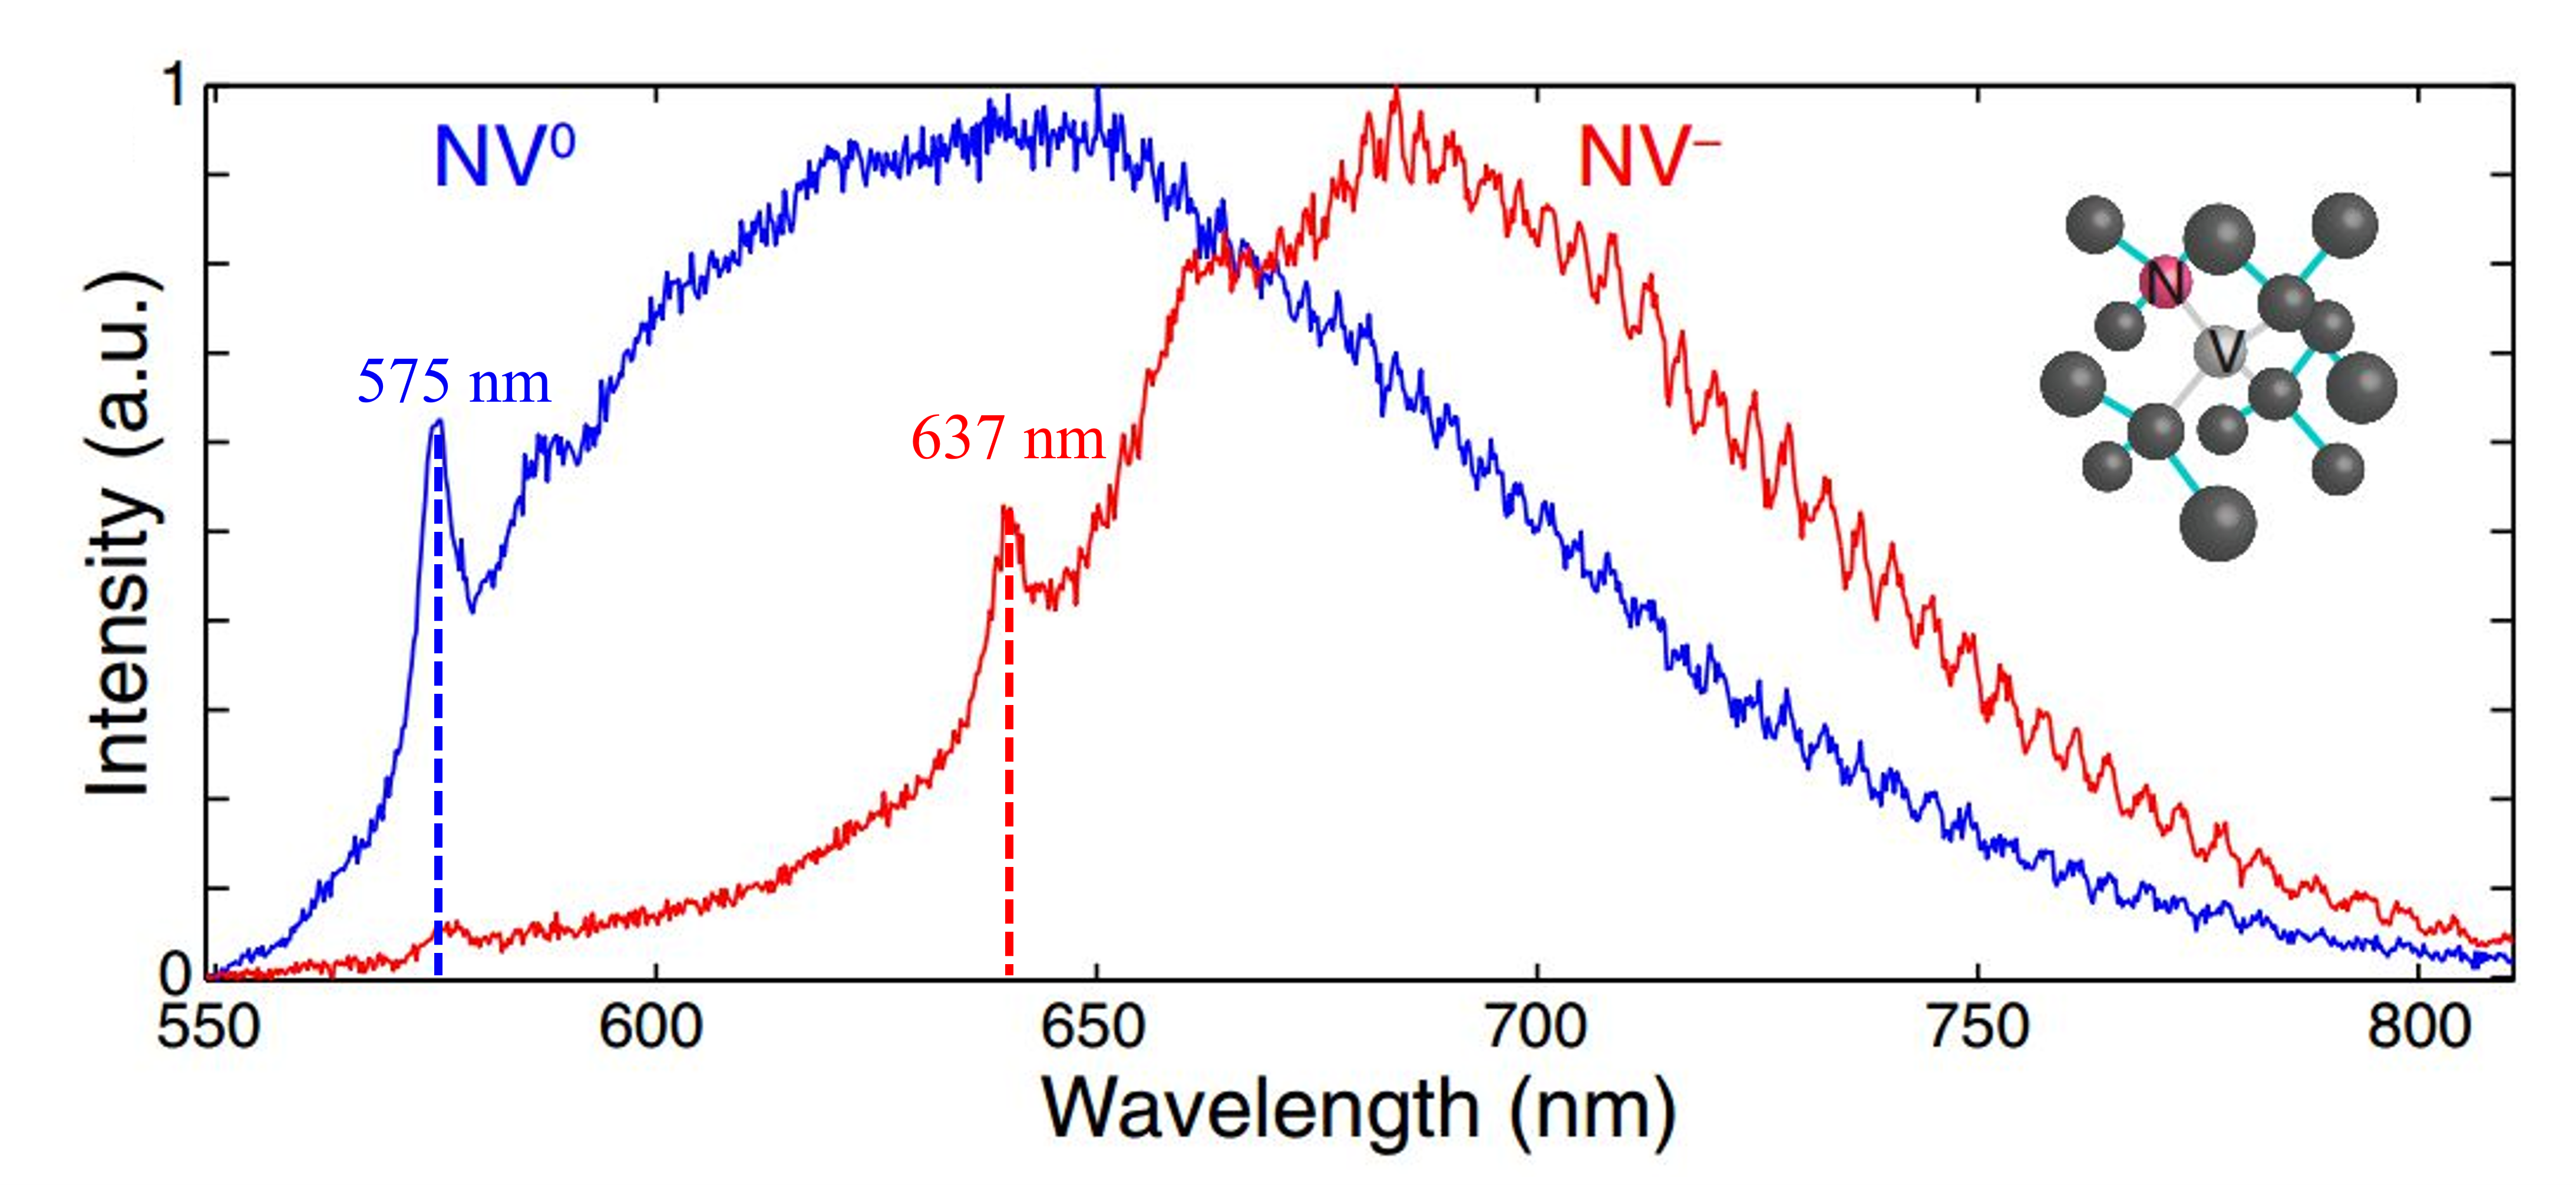
\includegraphics[width=1.0\textwidth]{figures/Chapter 1/NV Spectrum.png}
  \caption[NV Center在不同电荷态的时候的光谱图象]{NV Center在不同电荷态的时候的光谱图象,其中红色的线为NV$^-$的光谱,蓝色的线为NV$^0$的光谱,NV$^-$的零声子线位于637 nm处,NV$^0$的零声子线位于575 nm处\cite{karaveli2016modulation}。}
  \label{fig: NV Spectrum}
\end{figure}

\subsection{NV Center的电子能级结构}

\subsubsection{NV$^-$的电子能级结构}
对于我们最为关注的NV$^-$而言,其电子的能级结构可以用几个简单的三能级系统模型来描述,这个模型包括基态(ground state, GS)三重态(triplet)$^3A_2$(如图 \ref{fig: Electronic Structure}a)、激发态(excited state, ES)三重态$^3E$(如图 \ref{fig: Electronic Structure}b)和中间自旋单态(singlet state)。NV Center的负电荷状态NV$^-$是中性的NV$^0$捕获了一个电子形成的一个六电子缺陷能级结构,电子自旋量子数$S=1$的体系,这个结构可以通过各种方式在理论上进行模拟和验证,包括密度泛函理论、群论等方法\cite{lenef1996electronic,goss1997comment, maze2011properties, hossain2008ab, gali2009theory}。其中群论是一个非常强大且实用的工具,A. lenef和S. C. Rand在1996年的时候就通过群论预测了NV Center中的电子能级结构,其中较低的两个能级($a_1(1), a_2(2)$)有$a_1$对称性,较高的两个能级($e_x, e_y$)则在能量上退化兼并到关于$e$对称\cite{lenef1996electronic}。这些结论在后来人们拥有了超级计算机进行大规模密度泛函理论从头算(ab initio)的模拟的各项研究中被反复广泛的验证其可靠性和准确性\cite{gali2009theory, zou2023influence}。

在GS和ES的时候,三重态能级会发生零场劈裂(zero field splitting, ZFS)的现象,出现两个可以分辨的自旋能级$m_s=0$和$m_s=±1$,其中$m_s$为电子磁量子数。在GS的时候,其GS-ZFS的劈裂宽度大约为2870 \unit{\MHz},这使得其基态的自旋状态可以被微波(microwave, MW)所调控;而在ES的时候,其ES-ZFS约为GS-ZFS的一半,大概为1420 \unit{\MHz} \cite{gruber1997scanning,neumann2009excited}。

对于NV$^-$而言,缺陷能级中一共有六个价电子,在$^3A_2$基态的时候,$a_1(1), a_2(2)$能级都是被电子完全占据的,剩下的两个电子分别占据了$e_x, e_y$这两个能量较高的能级,便构成了$S=1$的自旋三重态。在$^3A_2$和$^3E$能级之间,电子可以发生较为明显的ZPL偶极跃迁,其在室温条件下,$a_2(2)$能级中自旋向下的电子吸收532 nm的绿光光子跃迁到被激发到$e_x$能级,然后退激发释放637 nm (1.945 \unit{\eV})的红光光子从而回到$^3A_2$基态,如图 \ref{fig: Electronic Structure}c所示。值得注意的是,在室温条件下,电子从$^3E$能级退激发到基态的过程中,有一部分情况会不可避免的和晶体声子产生相互作用,通过系统间交叉(intersystem crossing, ISC),从自旋单态的退激发到$^3A_2$,这个过程中不会辐射出可见光,如图 \ref{fig: Electronic Structure}c所示。

\begin{figure}
  \centering
  \includegraphics[width=1.0\textwidth]{figures/Chapter 1/Electronic Structure.png}
  \caption[NV$^-$的电子能级结构示意图]{NV$^-$的电子能级结构示意图,展示了带隙中间的缺陷能级:(a)$^3A_2$基态;(b)$^3E$激发态;(c)自旋三重态和ZPL跃迁过程,以及在自旋单态下的ISC作用\cite{staudacher2015nuclear}。}
  \label{fig: Electronic Structure}
\end{figure}

需要注意的一点是,图 \ref{fig: Electronic Structure}中所展示的NV Center的电子能级结构仅仅是一个简单的示意图,更加详细的细节,比如自旋单态ISC过程的能级结构、电子和氮核自旋之间超精细相互作用(hyperfine interaction)在这里并没有详细的给出,这些内容会在后续的章节中有所涉及。

因为金刚石中电子的自旋-翻转作用需要通过金刚石晶体中的声子的释放来进行能量交换,所以NV自旋态之间的弛豫时间$T_1$与声子态密度有关。由于金刚石的德拜温度(Debye temperature)较高,所以声子态密度在环境室温的情况下较小,因此NV Center有着较低的电子-声子耦合性,从而有着较长的$T_1$弛豫时间\cite{koizumi2008physics}。较长的$T_1$时间与金刚石中较弱的自旋-轨道作用密切相关,其使得NV自旋态之间产生微小的混合状态,这些自旋态又与电子-声子相互作用发生耦合,从而使得NV自旋态发生弛豫。另外,因为金刚石较宽的带隙,所以NV Center存在于带隙中的缺陷能级受到外界环境的干扰较小,因此有着较高的稳定性。金刚石的这些独特的性质使得其在室温条件下,对于缺陷能级的跃迁效应不会有额外的影响,让NV Center的量子效应在室温情况下仍然可以被观测到并可以被用于量子信息、量子精密测量等领域,这一点相比于其他的量子体系,比如超导量子比特(superconducting qubit)、离子阱(trapped ions)等体系,有着非常大的优势\cite{hu2023progress, acosta2013nitrogen}。

\subsubsection{NV$^0$的电子能级结构}
对于NV$^0$而言,其电子能级结构和NV$^-$有所不同,如图 \ref{fig: NV0 Electronic Structure}所示。相对于有两个额外的未成对电子组成电子自旋量子数$S=1$的NV$^-$,NV$^0$的外部仅有一个额外的未成对电子,在光学激发的情况下,NV$^0$的能级结构可能是自旋量子数为$S=\frac{1}{2}$的自旋二重态(spin doublet)或$S=\frac{3}{2}$的自旋四重态(spin quadruplet state)。由于电子顺磁共振(electron paramagnetic resonance, EPR)实验过程中的干扰,Jahn-Teller畸变的效应对于NV$^0$的自旋二重态的影响较大,因此中性电荷态的NV Center并不适合各种各样基于电子自旋相关的测量,所以绝大部分的研究都是基于NV$^-$的电子自旋态进行的\cite{gali2009theoryoftheneutral}。然而,NV$^0$的电子能级结构对于NV$^-$的电子能级结构的理解和研究仍然有着重要的意义,比如在NV$^-$的电子自旋态和氮核自旋态之间的超精细相互作用的研究中,NV$^0$的电子能级结构可以作为NV$^-$的电子能级结构的参考,从而可以更好地理解NV$^-$的电子能级结构\cite{gali2009theoryoftheneutral}。

\begin{figure}
  \centering
  \includegraphics[width=0.9\textwidth]{figures/Chapter 1/NV0 Electronic Structure.jpg}
  \caption[NV$^-$和NV$^0$的电子能级结构对比]{NV$^-$和NV$^0$的电子能级结构对比,a图和b图分别展示了NV$^-$和NV$^0$的基态、激发态、自旋单态的能级结构。图中分别NV$^-$和NV$^0$的ZPL能量,分别为1.945 eV(637 nm)和2.156 ev(575 nm),其中对于NV$^-$而言,自旋单态ISC过程的基态和激发态之间的能量差为1.190 eV(1041 nm)\cite{doherty2013nitrogen}。}
  \label{fig: NV0 Electronic Structure}
\end{figure}

本文的工作和研究主要依靠NV$^-$的基态和激发态自旋三重态,以及NV$^0$的基态和激发态的自旋双重态,包括他们的能级跃迁过程,因为这些决定了我们可以观测到的荧光效应,并由此来表征NV Center的各种性质。除此之外,这些荧光效应是光子激发电离过程的基础,因为它们在双光子激发自旋三重态和双重态的过程中,使得金刚石导带和价带的电子产生交换关联的效应,从而让荧光现象有着可观测的规律来让人们进行研究和应用\cite{aslam2013photo}。需要提到的一点是,对于ISC过程而言,也就是NV$^0$的自旋四重态和NV$^-$的自旋单态,在本文所研究的电荷态动力学这一关注点之下是可以忽略的,因为在目前的科学研究之中,这些状态时不参与NV Center的光致发光和光子激发电离的过程的。

\subsection{NV Center的光学和自旋性质}
对于单个NV Center而言,其光致发光的特性可以通过激光光子的吸收和发射来进行调控,在室温条件下作为一个在可见光波段的稳定的单光子发射源,这一点在量子信息和量子通信领域有着广泛的应用。NV Center的能级结构的一个重要的特征是其可以进行光学极化(optical polarization),也就是控制电子在不同的特定能级的分布率,如图 \ref{fig: Optical Properties}所示。

\begin{figure}
  \centering
  \includegraphics[width=1.0\textwidth]{figures/Chapter 1/Optical Properties.png}
  \caption[NV Center的电子能级结构和光学激发性质]{NV Center的电子能级结构和光学激发性质。(a)NV$^-$的基态具有沿着轨道A$_2$对称的自旋三重态,在光学跃迁激发的过程中,有一定概率会从自旋单态的亚稳态从激发态回到基态;(b)零外场的情况下,自旋-自旋(spin-spin)和自旋-轨道(spin-orbit)各自之间的相互作用使得基态和激发态出现了精细结构(fine structure);(c)(d)激发态和基态中简并的能级在外磁场的作用下发生劈裂。}
  \label{fig: Optical Properties}
\end{figure}

图(a)中,基态的电子可以通过非共振激发(光子的波长小于637 nm的ZPL波长)或者共振激发(光子的波长为637 nm的ZPL波长)被激发到激发态的三重态上,激发态的自旋三重态由于轨道双重态的作用,使得激发态存在六个能级。在室温下,通常利用532 nm的绿色激光将电子从基态激发到激发态六个能级的其中一个,这个过程是通过声子边带(phonon-sideband, PSB)非共振激发。由于自旋守恒跃迁(spin-conserving transitions)的效应,基态$m_s=\pm 1$能级的电子会被激发到激发态的$m_s=\pm 1$能级,这些电子会倾向于产生Intersystem Crossing(ISC)现象,由$^1A_1$和$^1E$的自旋单态亚稳态能级回到$m_s=0$的基态,这个过程不会发射可见光,单光子计数器的计数率会下降,这也是利用532 nm的激光对NV Center自旋状态进行读出和初始化的原理。图(b)中,零场状态下,基态的三重态分裂成$m_s = 0$能级和两个简并的能量相同的$m_s=\pm 1$能级,它们之间的能量差是2.88 GHz,因此可以利用微波进行对NV Center的自旋态进行调控。图(c)和(d)中,NV的$C_{3v}$轴向外磁场的作用下,基态和激发态的能级都会发生劈裂,这个劈裂的宽度和沿轴向的外磁场强度成正比,这也是利用NV Center进行磁场测量的原理。如果外磁场方向不呈NV的$C_{3v}$轴向,那么基态NV Center的自旋态会出现基态能级反交叉(ground-state level anticrossing)效应,使得荧光计数率的下降,在实验上通常利用这个效应来判断该亮点是否为NV Center。

就ISC效应而言,需要补充说明的一点是,在激发的时候,基态自旋状态为$m_s = 0$的电子会被激发到激发态的$m_s = 0$状态,这个时候不会趋向于产生ISC效应经过自旋单态,电子会从激发态的自旋三重态直接退激发回到基态的自旋三重态,在这个过程中会发射红光光子。总而言之,NV Center基态的自旋三重态可以被532 nm的绿色激光极化,并通过退激发所发出的红光进行读出。对于NV Center基态的自旋状态而言,我们可以通过特定频率的微波进行调控,也就是单电子自旋共振(Electron Spin Resonance, ESR)技术。

\section{NV Center电子自旋的调控}

NV Center电子自旋的调控方式ESR的原理类似于核磁共振(Nuclear Magnetic Resonance, NMR),即只是将关注的实验对象从原子核换成了电子,所以绝大部分理论和方法都是共通的。其中,区别最大的地方就是电子自旋的旋磁比(gyromagnetic ratio)为$\gamma_e=2.8$ MHz/G,比核自旋旋磁比大三个数量级,所以电子自旋更容易收到外界环境的影响,比如外界的磁噪音,从而发生退相干,丢失其携带的量子信息。当然,当NV Center作为传感用途的时候,其电子自旋态对于环境的敏感性也使得它成为一种灵敏度极高的量子精密测量器件。

\subsection{NV Center的哈密顿量}

正如前文所提到的,在NV Center处于基态的时候,其电子自旋并没有非常明显的自旋轨道耦合效应(spin-orbit coupling),因此其自旋动力学基本上是由其零场劈裂(zero-field splitting, ZFS)、电子Zeeman项、电子自旋和氮核自旋的超精细相互(hyperfine interaction)作用等因素所影响的,其哈密顿可以写成这样的形式:
\begin{equation}
  \mathcal{H}_{NV} = \mathcal{H}_{ZFS}+\mathcal{H}_{eZ}+\mathcal{H}_{hf}
  \label{equ: NV Hamiltonian}
\end{equation}
其中,$\mathcal{H}_{ZFS}$为ZFS项的哈密顿量,$\mathcal{H}_{eZ}=-\mu_eB$为电子Zeeman项在外磁场$B$作用下的哈密顿量,$\mathcal{H}_{hf}$是电子自旋和氮核自旋相互作用的超精细作用项的哈密顿量。

\subsection{光探测磁共振}

光探测磁共振(Optically Detected Magnetic Resonance, ODMR)技术是指原子、分子的光学频率的共振与射频或微波频率的磁共振同时发生的双共振现象。对于NV Center而言,就是利用微波使其电子自旋在ZFS劈裂的能级之间进行调控,然后通过读取光子数据在不同微波频率处的对比度来确定共振谱的技术。在实验中,ODMR又分为连续ODMR(Continuous Wave-ODMR,CW-ODMR)和脉冲ODMR(Pulsed ODMR)两种形式,下面进行分别介绍。

\subsubsection{CW-ODMR}

CW-ODMR是最为基础的序列测量,其基本原理是在持续激发和读出的过程中,施加连续的微波信号,测试不同频率的微波信号激发的情况下,计数率的变化,从而得到NV Center在基态的三重态之间的能量差异所导致的共振频率,测量序列如图 \ref{fig: CW-ODMR_seq}所示。
\begin{figure}
  \centering
  \includegraphics[width=1.0\textwidth]{figures/Chapter 1/CW-ODMR_seq.png}
  \caption[CW-ODMR的测量序列]{CW-ODMR的测量序列,532 nm的激光、微波和单光子计数器读出从始至终一直保持开启的持续状态。}
  \label{fig: CW-ODMR_seq}
\end{figure}
具体来说,在持续的532 nm激光的激发下,NV Center会处一个比较亮的状态,单光子计数器的读数较高,这是因为532 nm激光的激发会使得电子的自旋被持续性的初始化到$m_s=0$的态上,而$m_s=0$的态在被激发的后,退激发的时候不会发生ISC效应,从而会发射红光光子。当受到能量和$m_s=\pm1$与$m_s=0$之间能量差值相同的微波的时候,电子自旋会发生共振,也就是布居数分布从$m_s=0$被翻转到$m_s=\pm1$,这使得计数率下降。
\begin{figure}
  \centering
  \includegraphics[width=1.0\textwidth]{figures/Chapter 1/CW-ODMR_results.png}
  \caption[CW-ODMR的测量结果]{CW-ODMR的测量结果,(a)零场状态下CW-ODMR的测量结果,dip的位置在2.87 GHz处,对比度约为25.4 \%,为$m_s=\pm1$的双重简并态;(b)外磁场沿NV轴向的情况下CW-ODMR的测量结果,两个dips的平均位置大约在2.87 GHz处,但是每个峰的对比度变小。}
  \label{fig: CW-ODMR_results}
\end{figure}
如图 \ref{fig: CW-ODMR_results}(a)所示,展示了在零外场状态下的CW-ODMR的实验结果,可以看到微波频率为2.87 GHz处,出现一个对比度约为25.4 \%的dip,这是因为NV Center的自旋态发生了共振,$m_s=\pm1$态的电子被激发后,退激发的过程中不会发出650-800 nm区间的可见光,因此荧光效应在共振频率的时候会减弱。在图 \ref{fig: CW-ODMR_results}(b)中,展示了在外磁场沿着NV轴向的情况下的CW-ODMR的实验结果,可以看到在这种情况下,出现了两个dips,每个dip的对比度相较于零外场的情况下变小,这是因为外磁场的作用使得NV Center的$m_s=\pm1$态发生劈裂,从而在微波扫频的过程中出现了两个明显的dips,dips之间的距离和沿NV轴向的磁场强度成正比,这也是利用NV Center进行磁场测量的原理之一。

\subsubsection{Pulsed ODMR}

由于宽频的微波源的精度和稳定性有限,CW-ODMR的测量精度和分辨率都有所限制,因此在实验中通常会使用脉冲ODMR(Pulsed ODMR)技术,这种技术可以通过微波源提供一个基础频率,精细的频率调控通过任意波形发射器(Arbitrary Waveform Generator, AWG)脉冲序列的方式来进行NV Center的自旋态的调控,从而可以得到更高的测量精度和分辨率。脉冲ODMR的测量序列如图 \ref{fig: Pulsed ODMR_seq}所示。

\begin{figure}
  \centering
  \includegraphics[width=1.0\textwidth]{figures/Chapter 1/Pulsed ODMR_seq.png}
  \caption[Pulsed ODMR的测量序列]{Pulsed ODMR的测量序列,532 nm的激光、微波和单光子计数器读出按照时间序列交替进行。}
  \label{fig: Pulsed ODMR_seq}
\end{figure}

Pulsed ODMR测量序列中,先用532 nm的激光对NV Center进行初始化,将所有的电子自旋都初始化到$m_s=0$态;然后利用脉冲微波序列对电子的自旋状态进行调控,使得其翻转到指定的状态;最后通过532 nm的激光对自旋态进行读出,同时通过APD进行计数统计。在这里需要注意一点的是,我们需要选择测量区间和参考区间,通过对比两个区间的计数率,可以得到NV Center的自旋态的信息,如图 \ref{fig: mes_ref}所示。

\begin{figure}
  \centering
  \includegraphics[width=0.6\textwidth]{figures/Chapter 1/mes_ref.png}
  \caption[Pulsed ODMR的测量读出]{Pulsed ODMR的测量读出,NV Center处于$|0\rangle$态的时候,计数率较高;NV Center处于$|1\rangle$态的时候,计数率较低;最后所有的电子自旋状态都被初始化到$|0\rangle$态\cite{staudacher2015nuclear}。}
  \label{fig: mes_ref}
\end{figure}

在NV Center经过Pulsed MW调控后第一次激发的时候,处于$|0\rangle$态的电子产生的荧光计数率较高,而处于$|1\rangle$态的电子产生的荧光计数率较低。对于NV Center的电子而言,每轮的激发和退激发的过程是需要一定的时间,这也就是测量窗口的时间长度,超过这个时间之后,所有的电子都会被初始化到$|0\rangle$态,荧光计数率恢复到较高的状态。我们需要通过测量窗口(mes)内荧光计数率的降低和完全初始化后荧光计数率(ref)进行对比,即可得出NV Center的自旋态的信息。通常这个序列会重复多次,从而降低测量的误差,得到更加准确的结果。如图 \ref{fig: Pulsed ODMR_results}(a)所示,可以看到$^{14}N$的超精细相互作用导致的三个dips,相邻的dips之间的距离大概是2 MHz。如图 \ref{fig: Pulsed ODMR_results}(b),展示了该NV Center周围存在$^{13}C$的spin bath的情况下的Pulsed ODMR的测量结果,$^{13}C$ spin bath的存在会导致$^{14}N$的超精细相互作用的能级发生劈裂,产生六个能级,其中有两组重叠了两个能级的状态,最后测量得到四个dips,其中两个有能级重叠的dips较宽。

\begin{figure}
  \centering
  \includegraphics[width=1.0\textwidth]{figures/Chapter 1/Pulsed ODMR_results.png}
  \caption[Pulsed ODMR的测量结果]{Pulsed ODMR的测量结果,(a)零场状态下Pulsed ODMR的测量结果,周围不存在$^{13}C$的spin bath外场,出现了三个dips;(b)周围存在$^{13}C$的spin bath外场作用下的Pulsed ODMR的测量结果,出现了六个dips,其中有两组重叠了两个dips的较宽的dips,最后观测得到的就是4个dips。}
  \label{fig: Pulsed ODMR_results}
\end{figure}

\subsection{NV Center电子自旋的拉比振荡}

拉比振荡(Rabi oscillation)是量子力学中的一种现象,描述了一个处于两个能级之间的量子系统在外部激励下的振荡行为。这个现象是由Isidor Rabi在20世纪30年代首次提出并研究的,因此得名。拉比振荡通常发生在一个由两个能级组成的系统中,例如一个原子或者一个量子比特。这两个能级分别对应于系统的不同的量子态,在NV Center的电子自旋中,就是基态的$m_s=0$和$m_s = \pm1$的两个能级之间。在拉比振荡的过程中,系统会在这两个能级之间来回转换。拉比振荡的起因是外部激励,通常是通过一个恒定频率的电磁场(微波源)来实现。当外部电磁场与系统的共振频率匹配时,能级之间的跃迁会被促发,导致系统从一个能级跃迁到另一个能级。然而,由于量子干涉的效应,系统并不会一直保持在新的能级上,而是会在不同的能级之间进行振荡。这种振荡行为可以用数学上的波动方程来描述,通常采用薛定谔方程或者旋转波近似来处理。拉比振荡的频率由外部激励的强度和频率以及系统内部的能级差决定。在实验中,可以通过改变外部激励的参数来调控拉比振荡的频率和幅度。

如图 \ref{fig: Rabi Oscillation}所示,可以看到在不同的施加时间下,NV Center的电子自旋在两个能级之间发生了振荡,对于NV Center的电子自旋而言,可以通过Pulsed ODMR测量来使电子在两个能级之间实现Rabi oscillation,在改变微波的施加时间的过程中,记录荧光计数率的变化可以得到NV Center的拉比振荡的频率和幅度,从而得到特定微波功率下电子自旋$\pi$-pulse的长度,也就是在Bloch Sphere之中,自旋矢量旋转$\pi$所需施加微波时间,用于精确地调控电子自旋。

\begin{figure}
  \centering
  \includegraphics[width=1.0\textwidth]{figures/Chapter 1/Rabi Oscillation.png}
  \caption[Rabi Oscillation示意图]{Rabi Oscillation示意图。(a)NV Center基态(Ground State,GS)和激发态(Excited State,ES)的自旋三重态和亚稳态(Metastable State,MS)及其跃迁过程和微波调控调控的示意图。(b)NV Center电子自旋三重态和读出发光的情况。(c)NV Center电子自旋量子态在Bloch Sphere中的表现形式,北极为$m_s=0$态,南极为$m_s=\pm1$态,通过$\pi_x$或$\pi_y$微波脉冲可以将矢量指向翻转180°,在$m_s=0$和$m_s=\pm1$之间转换。(d)连续微波CW-ODMR测量结果。(e)NV Center电子自旋的Rabi Oscillation曲线。}
  \label{fig: Rabi Oscillation}
\end{figure}
图 \ref{fig: Rabi Oscillation} (a)和(b)中可以看到,NV Center被激光激发后,自旋处于$m_s=0$状态的电子回到基态的时候会发射可见光,被单光子计数器探测到发光现象;而自旋处于旋处于$m_s=\pm1$状态的电子会经过MS回到基态,在这个过程中不会发射可见光光子,从而处于黑暗的状态。图 \ref{fig: Rabi Oscillation} (d)中展示了连续微波CW-ODMR的测量结果,当微波频率和零场劈裂的频率2.87 GHz相同的时候,电子自旋会发生共振,自旋状态从$m_s=0$被翻转到$m_s=\pm1$,这时候用激光去激发,会检测到计数率下降,产生了dip。图 \ref{fig: Rabi Oscillation} (e)中展示了NV Center电子自旋的Rabi Oscillation曲线,可以看到在不同的微波施加时间下,NV Center的电子自旋在两个能级之间发生了振荡,通过改变微波的持续时间,可以使Bloch Sphere中的自旋矢量翻转不同的角度,从而使得计数率随时间的变化出现正弦曲线的形状,每个周期的长度就是微波将自旋矢量翻转360°($2\pi$)所需的时间,通过Rabi Oscillation的测试可以得到当前NV Center在特定功率微波下$\pi$-pulse的长度,用于精确地调控电子自旋。实际在10 dBm微波功率下测试Rabi Oscillation的结果如图 \ref{fig: Rabi Result} 所示,(a)图展示了单光子计数器的计数率随着共振微波持续时间变化曲线和拟合结果,可以看到Rabi Oscillation的$2\pi$周期在97.6 $\pm$ 1.2 ns,(b)图展示了曲线数据进行快速傅里叶变换(Fast Fourier Transformation,FFT)的结果,可以看到仅在10 MHz附近出现一个比较明显的频率峰,这也是Rabi Oscillation的频率。需要注意的一点是,由于我们在进行微波调控的时候一般只会利用到$0-2\pi$的范围,所以我们也会关注拟合出的正弦曲线的相位信息,用于控制自旋态翻转到特定的位置。

\begin{figure}
  \centering
  \includegraphics[width=1.0\textwidth]{figures/Chapter 1/Rabi Result.png}
  \caption[Rabi Oscillation测试结果图]{Rabi Oscillation测试结果图。(a)计数率随着连续共振微波持续时间变化曲线和拟合结果;(b)曲线数据进行快速傅里叶变换的结果。}
  \label{fig: Rabi Result}
\end{figure}

\subsection{NV Center电子自旋的自由感应衰减}

NV Center的电子自旋态作为一种量子比特(qubit),其携带有量子信息的相干态会不可避免的受到环境噪声的影响,比如外界的磁场或温度的变化、内部同位素原子核(通常情况为金刚石中自然丰度为1.1 \%的$^{13}$C)的自旋浴(Spin Bath)作用、声子对电子自旋的影响等等。通常情况下,由于晶格振动产生的声子对电子自旋产生纵向弛豫(T$_1$,~10$^3$ s),由于核自旋感应产生的使NV发生退相干效应为横向弛豫(T$_{2}^{*}$,~ μs)。在低温的环境下,T$_1$>>T$_{2}^{*}$,因此我们主要考虑的是T$_{2}^{*}$的影响。在实验中,我们通常会通过自由感应衰减(Free Induction Decay,FID)来表示NV Center电子自旋的T$_{2}^{*}$时间,其测量序列也被称为Ramsey序列,如图 \ref{fig: FID_seq}所示,通过施加两个$\frac{\pi}{2}$脉冲,然后在两个脉冲之间施加不同的等待时间$\tau$,最后通过读出激光和单光子计数器来得到NV Center电子自旋的自由感应衰减曲线。

\begin{figure}
  \centering
  \includegraphics[width=1.0\textwidth]{figures/Chapter 1/FID_seq.png}
  \caption[Ramsey序列测试FID的过程]{Ramsey序列测试FID的过程,(a)微波序列的构成;(b)自旋状态矢量受到Ramsey序列的调控在Bloch Sphere上的变化过程\cite{新型扫描量子传感显微镜系统的研发与应用}。}
  \label{fig: FID_seq}
\end{figure}
Ramsey序列调控单NV电子自旋的主要的原理是,在利用连续的532 nm绿色激光将NV Center的电子自旋初始化到$m_s = 0$态后断开激光,先利用$\frac{\pi}{2}$的微波脉冲将电子从$|0\rangle$翻转到$\frac{|0\rangle+|-1\rangle}{2}$的叠加态,然后弛豫$\tau$的时间使其自由演化。然后再利用$\frac{\pi}{2}$或$\frac{3\pi}{2}$的微波脉冲(通常情况我们同时使用这两种脉冲,将测量的数据相减来降低误差)将剩余的有效相位信息转化为荧光强度的布居数来读出。

\begin{figure}
  \centering
  \includegraphics[width=1.0\textwidth]{figures/Chapter 1/FID Result.png}
  \caption[FID测试结果]{FID测试结果,(a)Ramsey序列作用下,读出荧光计数率随着弛豫时间的变化,两条曲线为读出前翻转$\frac{\pi}{2}$和$\frac{3\pi}{2}$的测量结果;(b)将翻转$\frac{\pi}{2}$和$\frac{3\pi}{2}$的测量结果作差得到的结果。}
  \label{fig: FID Result}
\end{figure}

如图 \ref{fig: FID Result}所示,为Ramsey序列测量FID的结果,由图中信息可以看到曲线有振荡失谐的现象产生,这是由于NV Center中的同位素氮原子核$^{14}$N或$^{15}$N与电子之间的超精细相互作用(Hyperfine Interaction)导致的。当我们考虑准静态相互作用过程的时候,核自旋spin bath的哈密顿量为:
\begin{equation}
  \begin{aligned}
    H_{bath} &= \beta S_z \\
    \beta &= \Sigma^n_iA_{\parallel}^i
  \end{aligned}
\end{equation}
因此,FID的衰减函数可以写成:
\begin{equation}
  \begin{aligned}
    f_{\beta}(t) &\approx \langle S_x(t) \rangle_{\beta} \approx \frac{1}{2}e^{-\frac{1}{2}b^2t^2} \\
    b &= \sqrt{\Sigma_i^n(A_{\parallel}^i)^2}
  \end{aligned}
\end{equation}
当考虑考虑噪声关联函数的时候:
\begin{equation}
  \begin{aligned}
    C(s)=b^2exp(-\frac{|s|}{t_c})
  \end{aligned}
\end{equation}
这个时候FID的衰减函数可以写成如下形式:
\begin{equation}
  \begin{aligned}
    f(t)=exp[-b^2t_c^2(\frac{t}{t_c}+e^{-\frac{t}{t_c}}-1)]
  \end{aligned}
\end{equation}
在准静态过程中,噪音的变化很慢($t\ll t_c$),也就是说在相干时间的尺度内基本不会发生变化,那么如图 \ref{fig: FID Functions}(a)所示,FID的衰减曲线呈高斯衰减的趋势,相干时间为$T_2 = \sqrt{2/b^2}$,其中b定义为spin-bath相互作用强度,$t_c$量化了核自旋的翻转效率(flip-flop rates),也就代表着噪声相关时间。与之相反的,在考虑噪声变化较快的情况下($t\gg t_c$),FID的衰减曲线呈指数衰减的趋势,如图 \ref{fig: FID Functions}(b)所示,这种情况下,相干时间为$T_2 = 1/b^2t_c$,也就是说在这种情况下,NV Center的电子自旋的相干时间主要受到spin-bath噪声的影响较大,退相干的速度较快。
\begin{figure}
  \centering
  \includegraphics[width=1.0\textwidth]{figures/Chapter 1/FID Functions.png}
  \caption[FID相干性衰减曲线]{FID相干性衰减曲线,两个图展示了不同情况下的计数率变化曲线,将翻转$\frac{\pi}{2}$和$\frac{3\pi}{2}$的测量结果作差得到的结果。(a)准静态过程中,噪音关联时间远大于相干时间尺度($t\ll t_c$),噪音的作用强度较强($b\gg 1/t_c$);(b)噪音快速变化的环境下,噪音关联时间远小于相干时间的尺度($t\gg t_c$),噪音的作用强度较弱($b\ll 1/t_c$)。}
  \label{fig: FID Functions}
\end{figure}

\subsection{NV Center电子自旋的自旋-回波和动力学解耦序列}
为了提高NV Center电子自旋的相干性,延长相干时间,提高读出和门操作的保真度,我们会运用动力学解耦序列(Dynamical Decoupling Sequence)来操控电子自旋实现特定的翻转。最常见的Dynamical Decoupling序列就是自旋-回波(Spin-echo)序列,也被成为Hahn-echo序列,由Erwin Hahn在1950年首次提出\cite{hahn1950spin}。其基本原理如图\ref{fig: Hahn Sequence},在电子自旋自由演化一段时间后,产生了退相干的相位,然后施加一个$\pi$脉冲,对相位在时间尺度上进行反演操作,从而使得之前产生的相位被抵消,恢复自旋相干性,延长相干时间。
\begin{figure}
  \centering
  \includegraphics[width=1.0\textwidth]{figures/Chapter 1/Hahn Sequence.png}
  \caption[Hahn-echo 序列]{Hahn-echo 序列,(a)在Hahn-echo序列作用下,电子自旋矢量在布洛赫球中的变化;(b)Hahn-echo序列的微波示意图,在中间$\tau/2$的位置插入了一个$\pi$脉冲。\cite{新型扫描量子传感显微镜系统的研发与应用}}
  \label{fig: Hahn Sequence}
\end{figure}

在应用自旋-回波序列之后,退相干函数中加入了一项滤波项:
\begin{equation}
  \xi_{echo}(t)=\left\{
  \begin{array}{rcl}
  +1 & & {t \in [0, \tau]}\\
  -1 & & {t \in [\tau, 2\tau]}
  \end{array} \right.
  \end{equation}
因此,退相干衰减函数的表达形式可以写为:
\begin{equation}
  f(t) = exp[-b^2t_c^2(\frac{t}{t_c}+4e^{-\frac{t}{2t_c}}-e^{-\frac{t}{t_c}}-3)]
\end{equation}
自旋-回波序列的前提使环境噪声是准静态变化的,也就是噪声变化的时间尺度要大于序列操控的时间$\tau$,自旋-回波序列才能对相干时间起到较好的提升作用。为了区分FID自由演化下的相干时间,经过Dynamical Decouping序列处理后的相干时间定义为$T_2^*$。如图 \ref{fig: Hahn Functions}(a)中的曲线所示,在准静态过程中,噪音关联时间远大于相干时间尺度($t\ll t_c$),其衰减函数可以简化为$f(t) = exp(-\frac{b^2t^3}{12t_c})$,因此相干时间$T_2^*=\sqrt[3]{\frac{12t_c}{b^2}}$,其相干时间明显长于同等情况下的$T_2$。然而对于快速变化的噪声环境,如图 \ref{fig: Hahn Functions}(b)中的曲线所示,噪音关联时间远小于相干时间的尺度($t\gg t_c$),其衰减函数可以简化为$f(t) = exp(-b^2t_ct)$,因此相干时间$T_2^*=(b^2t_c)^{-1}\ \textasciitilde \ T_2$,其相干时间和同等情况下的$T_2$相近,也是就自旋回波序列无法让相干时间实现较为明显的提升。
\begin{figure}
  \centering
  \includegraphics[width=1.0\textwidth]{figures/Chapter 1/Hahn Functions.png}
  \caption[Hahn-echo 序列作用下的相干性衰减曲线]{Hahn-echo 序列作用下的相干性衰减曲线,两个图展示了不同情况下的计数率变化曲线,将翻转$\frac{\pi}{2}$和$\frac{3\pi}{2}$的测量结果作差得到的结果。(a)准静态过程中,噪音关联时间远大于相干时间尺度($t\ll t_c$),噪音的作用强度较强($b\gg 1/t_c$);(b)噪音快速变化的环境下,噪音关联时间远小于相干时间的尺度($t\gg t_c$),噪音的作用强度较弱($b\ll 1/t_c$)。}
  \label{fig: Hahn Functions}
\end{figure}
除此之外,我们还可以通过其他的Dynamical Decoupling序列来提高NV Center电子自旋的相干时间,比如Carr-Purcell-Meiboom-Gill(CPMG)序列、Uhrig Dynamical Decoupling(UDD)序列、XY8序列等等,这些序列的原理和应用类似于Hahn-echo,本质上是不断地快速重复Hahn-echo序列,使其在间隔的退相干尺度$\tau$时间减小,尽可能地小于噪音环境的变化尺度,可以尽量接近准静态噪声的过程,从而提高NV Center电子自旋的相干时间。在这些重复序列中,退相干函数可以粗略地写成$f(t)=exp[-\frac{1}{N^2}(\frac{t}{T_2})^3]$,相干时间和$N^{2/3}$成正相关的关系,也就是说通过增加序列的重复次数,可以提高NV Center电子自旋的相干时间。如图 \ref{fig: XY8 Sequence}所示,可以看到XY8序列重复次数N越大,其保持高信号强度的时间越长,相干时间也就越长。除此之外,XY8序列通过交替施加$\pi_x$和$\pi_y$,修正了微波脉冲的在$S_x$和$S_y$方向可能存在的轻微失相,进一步地延长了相干时间。但是$\pi$ pulse重复次数N不可能无限制的增大,因为在间隔时间$\tau$逐渐减小的时候,$\pi$ pulse的持续时间相对于间隔的演化时间$\tau$就不可忽略,所以其状态的保真度会降低,如图 \ref{fig: XY8 Sequence}(d)所示。同时,N的选取也要尽量避免其频率和周围核自旋的Lamor频率接近,使得核自旋被共振驱动,对spin bath产生额外的影响。QuTech的研究人员通过XY8序列将NV Center的电子自旋时间提高了近三个数量级\cite{abobeih2018one}。
\begin{figure}
  \centering
  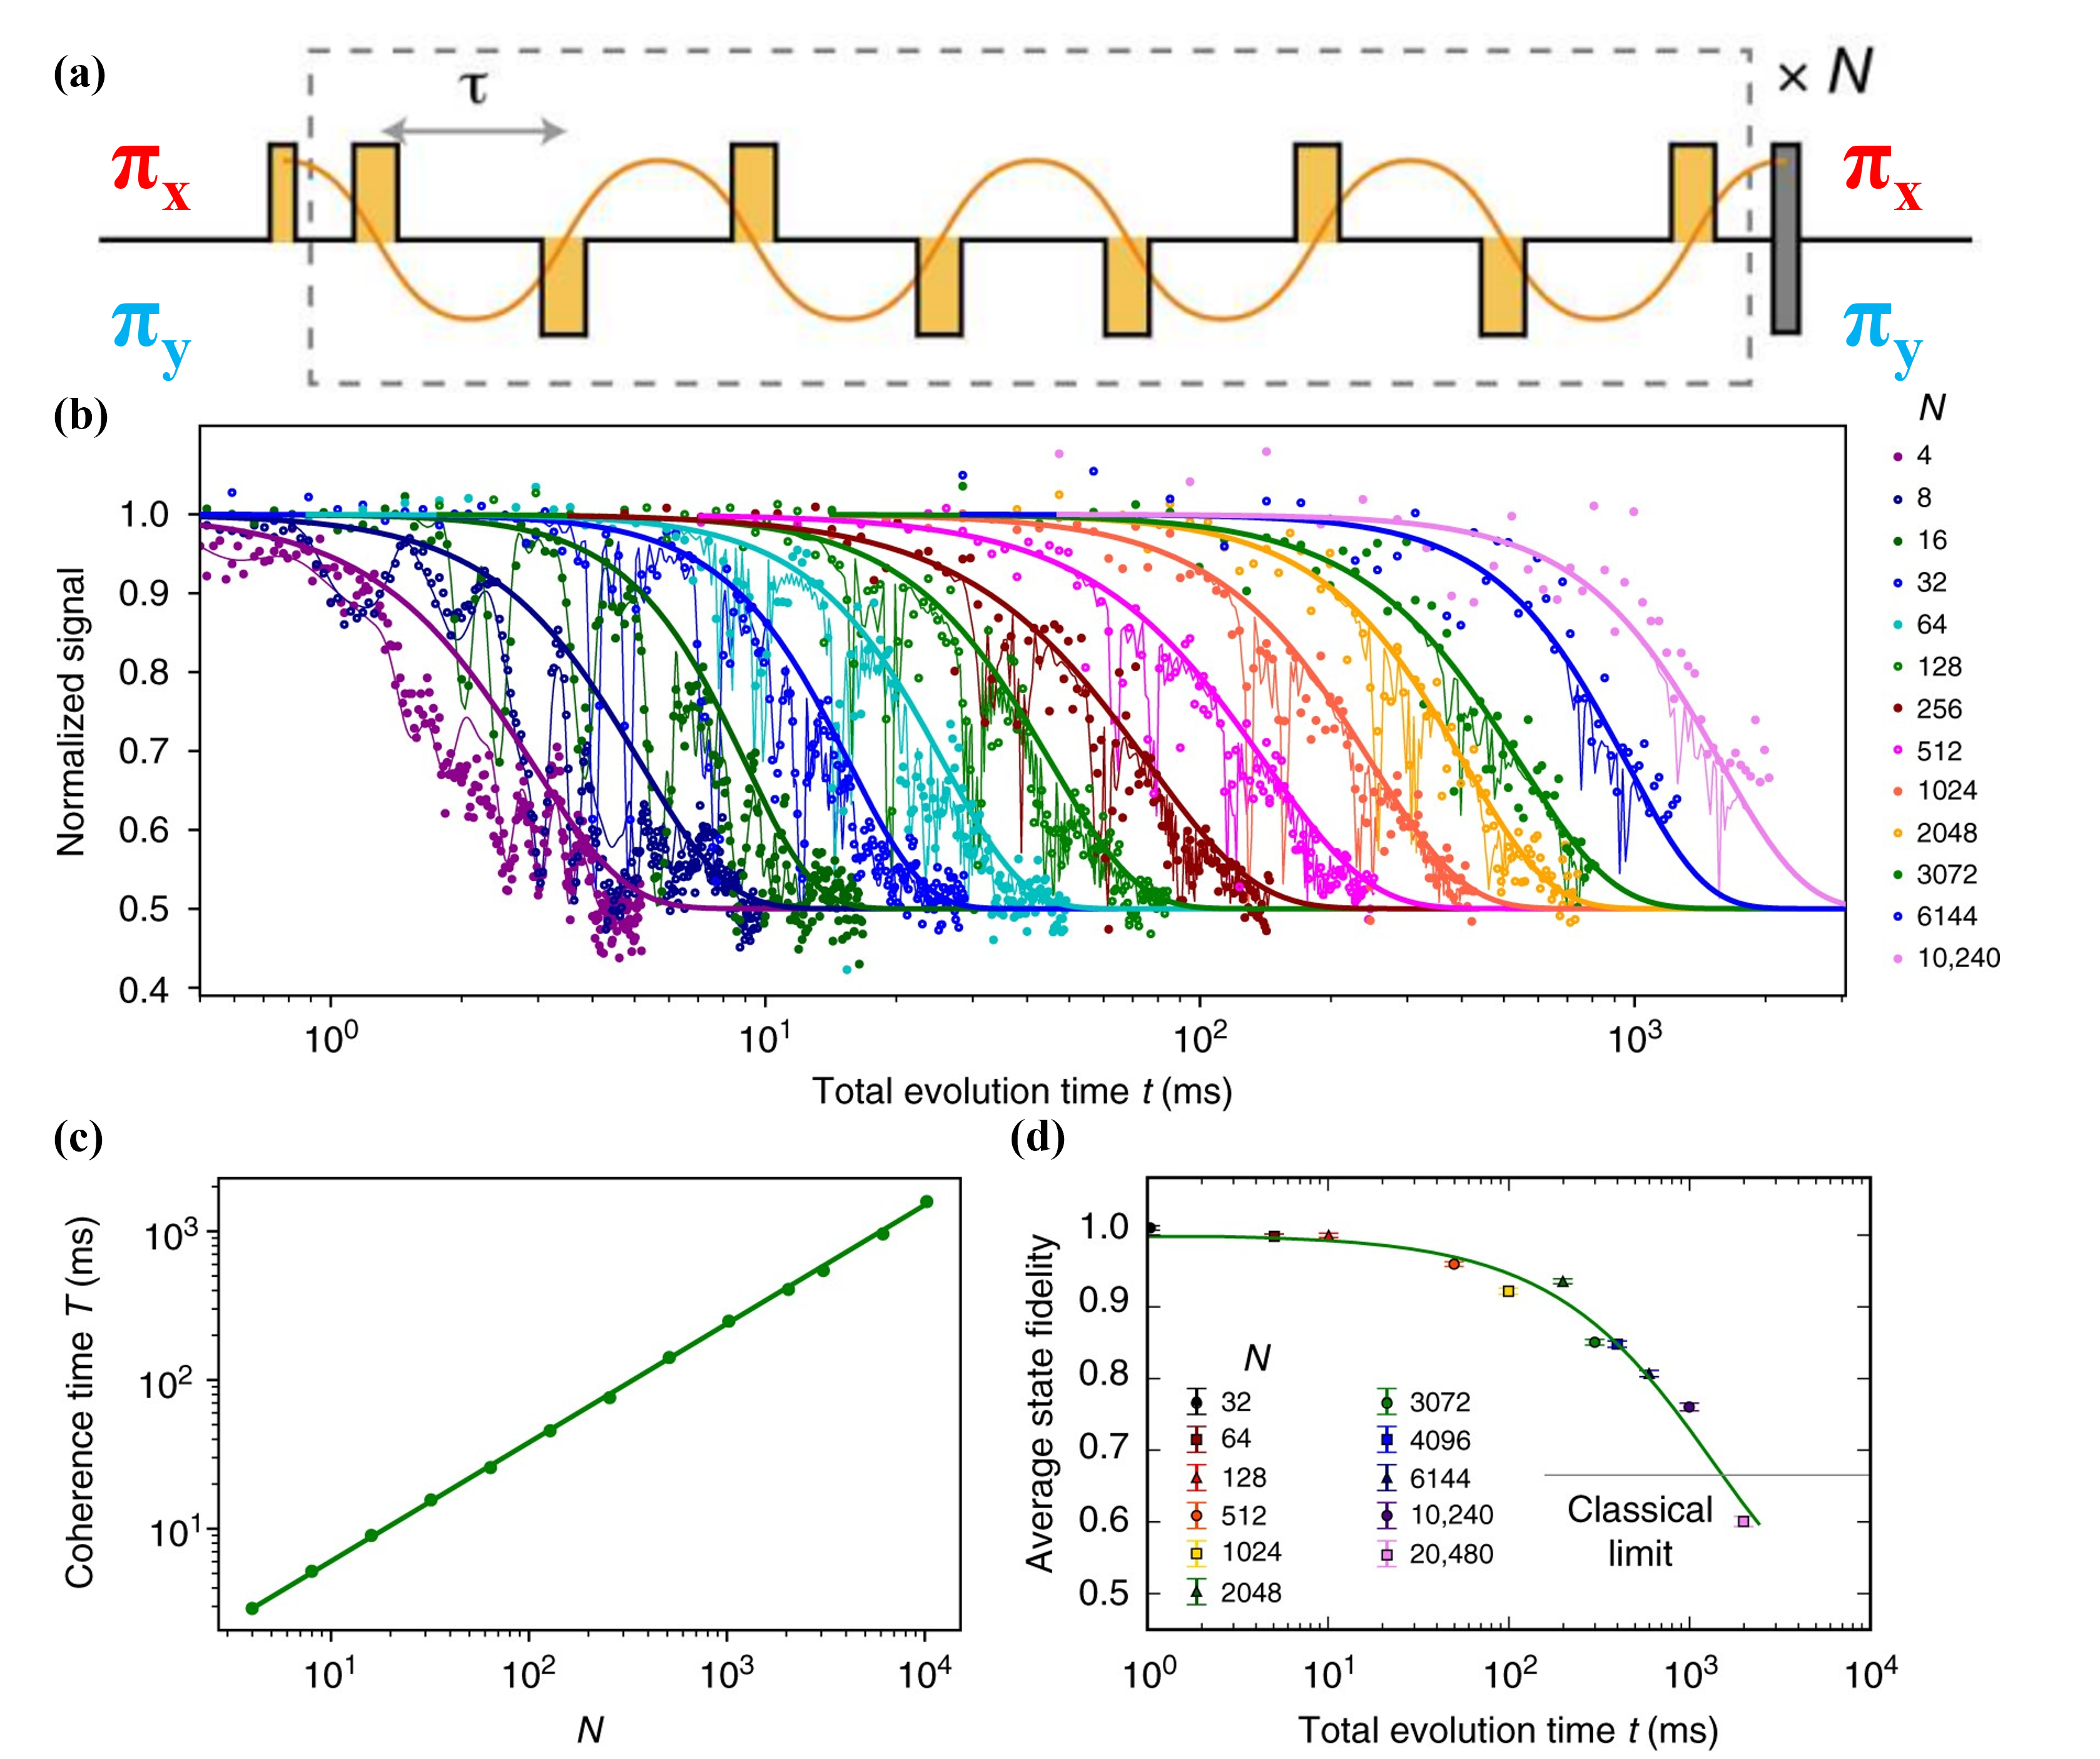
\includegraphics[width=1.0\textwidth]{figures/Chapter 1/XY8 Sequence.png}
  \caption[XY8 序列作用下的相干性衰减曲线和相干时间]{XY8 序列作用下的相干性衰减曲线和相干时间。(a)XY8序列微波操控示意图;(b)不同的序列重复次数N的XY8序列下,观测到的信号强度随着时间的变化;(c)相干时间和序列重复次数N之间的关系;(d)演化时间和状态保真度之间的变化关系。\cite{abobeih2018one}}
  \label{fig: XY8 Sequence}
\end{figure}

\section{共聚焦显微镜系统实验平台的设计与搭建}
\subsection{共聚焦显微镜的基本原理}
实验室中常见的光学显微镜是通过光源发出自然光(白光)投射到被测样品上,样品的反射或透射光被物镜聚焦到目镜上,通过目镜观察到被测样品的图像。这种显微镜的分辨率受到可见光的波长的限制,通常在0.2 $\mu m$左右。为了提高显微镜的分辨率,人们提出了共聚焦显微镜(Confocal Microscopy)的概念,通过在显微镜中加入共聚焦系统,可以使得显微镜的分辨率提高到0.1 $\mu m$以下。共聚焦显微镜的基本原理是通过激光光源发出的激光束照射到样品上,样品的受到激光的激发后,在退激发的过程中会产生荧光效应释放出光子,被物镜聚焦到探测器上,并将信息传回到电脑。共聚焦显微镜的分辨率受到激光波长和物镜规格的限制,通常能在0.1 $\mu m$以下。共聚焦显微镜的优点是可以观察到样品的表面形貌和内部结构,实现三维的成像,非接触式无损的高分辨率、高灵敏度、高对比度的观察。

对于NV Center而言,由于基态能级结构的电子能被绿光激发,并在退激发的过程中发射声子边带的红光光子,所以共聚焦显微镜的原理可以用于对金刚石中的NV Center进行表征和检测,通过激光的聚焦和荧光的检测,可以实现对不同深度NV Center的三维定位和成像。一般来说,共聚焦显微镜有以下几个主要的部分:激光光源、激光束聚焦系统、样品台、物镜、探测器、数据采集系统等等。平台的构建也有多种方案,通过镜头的放置方式和扫描的运行方式来区分。
\begin{figure}
  \centering
  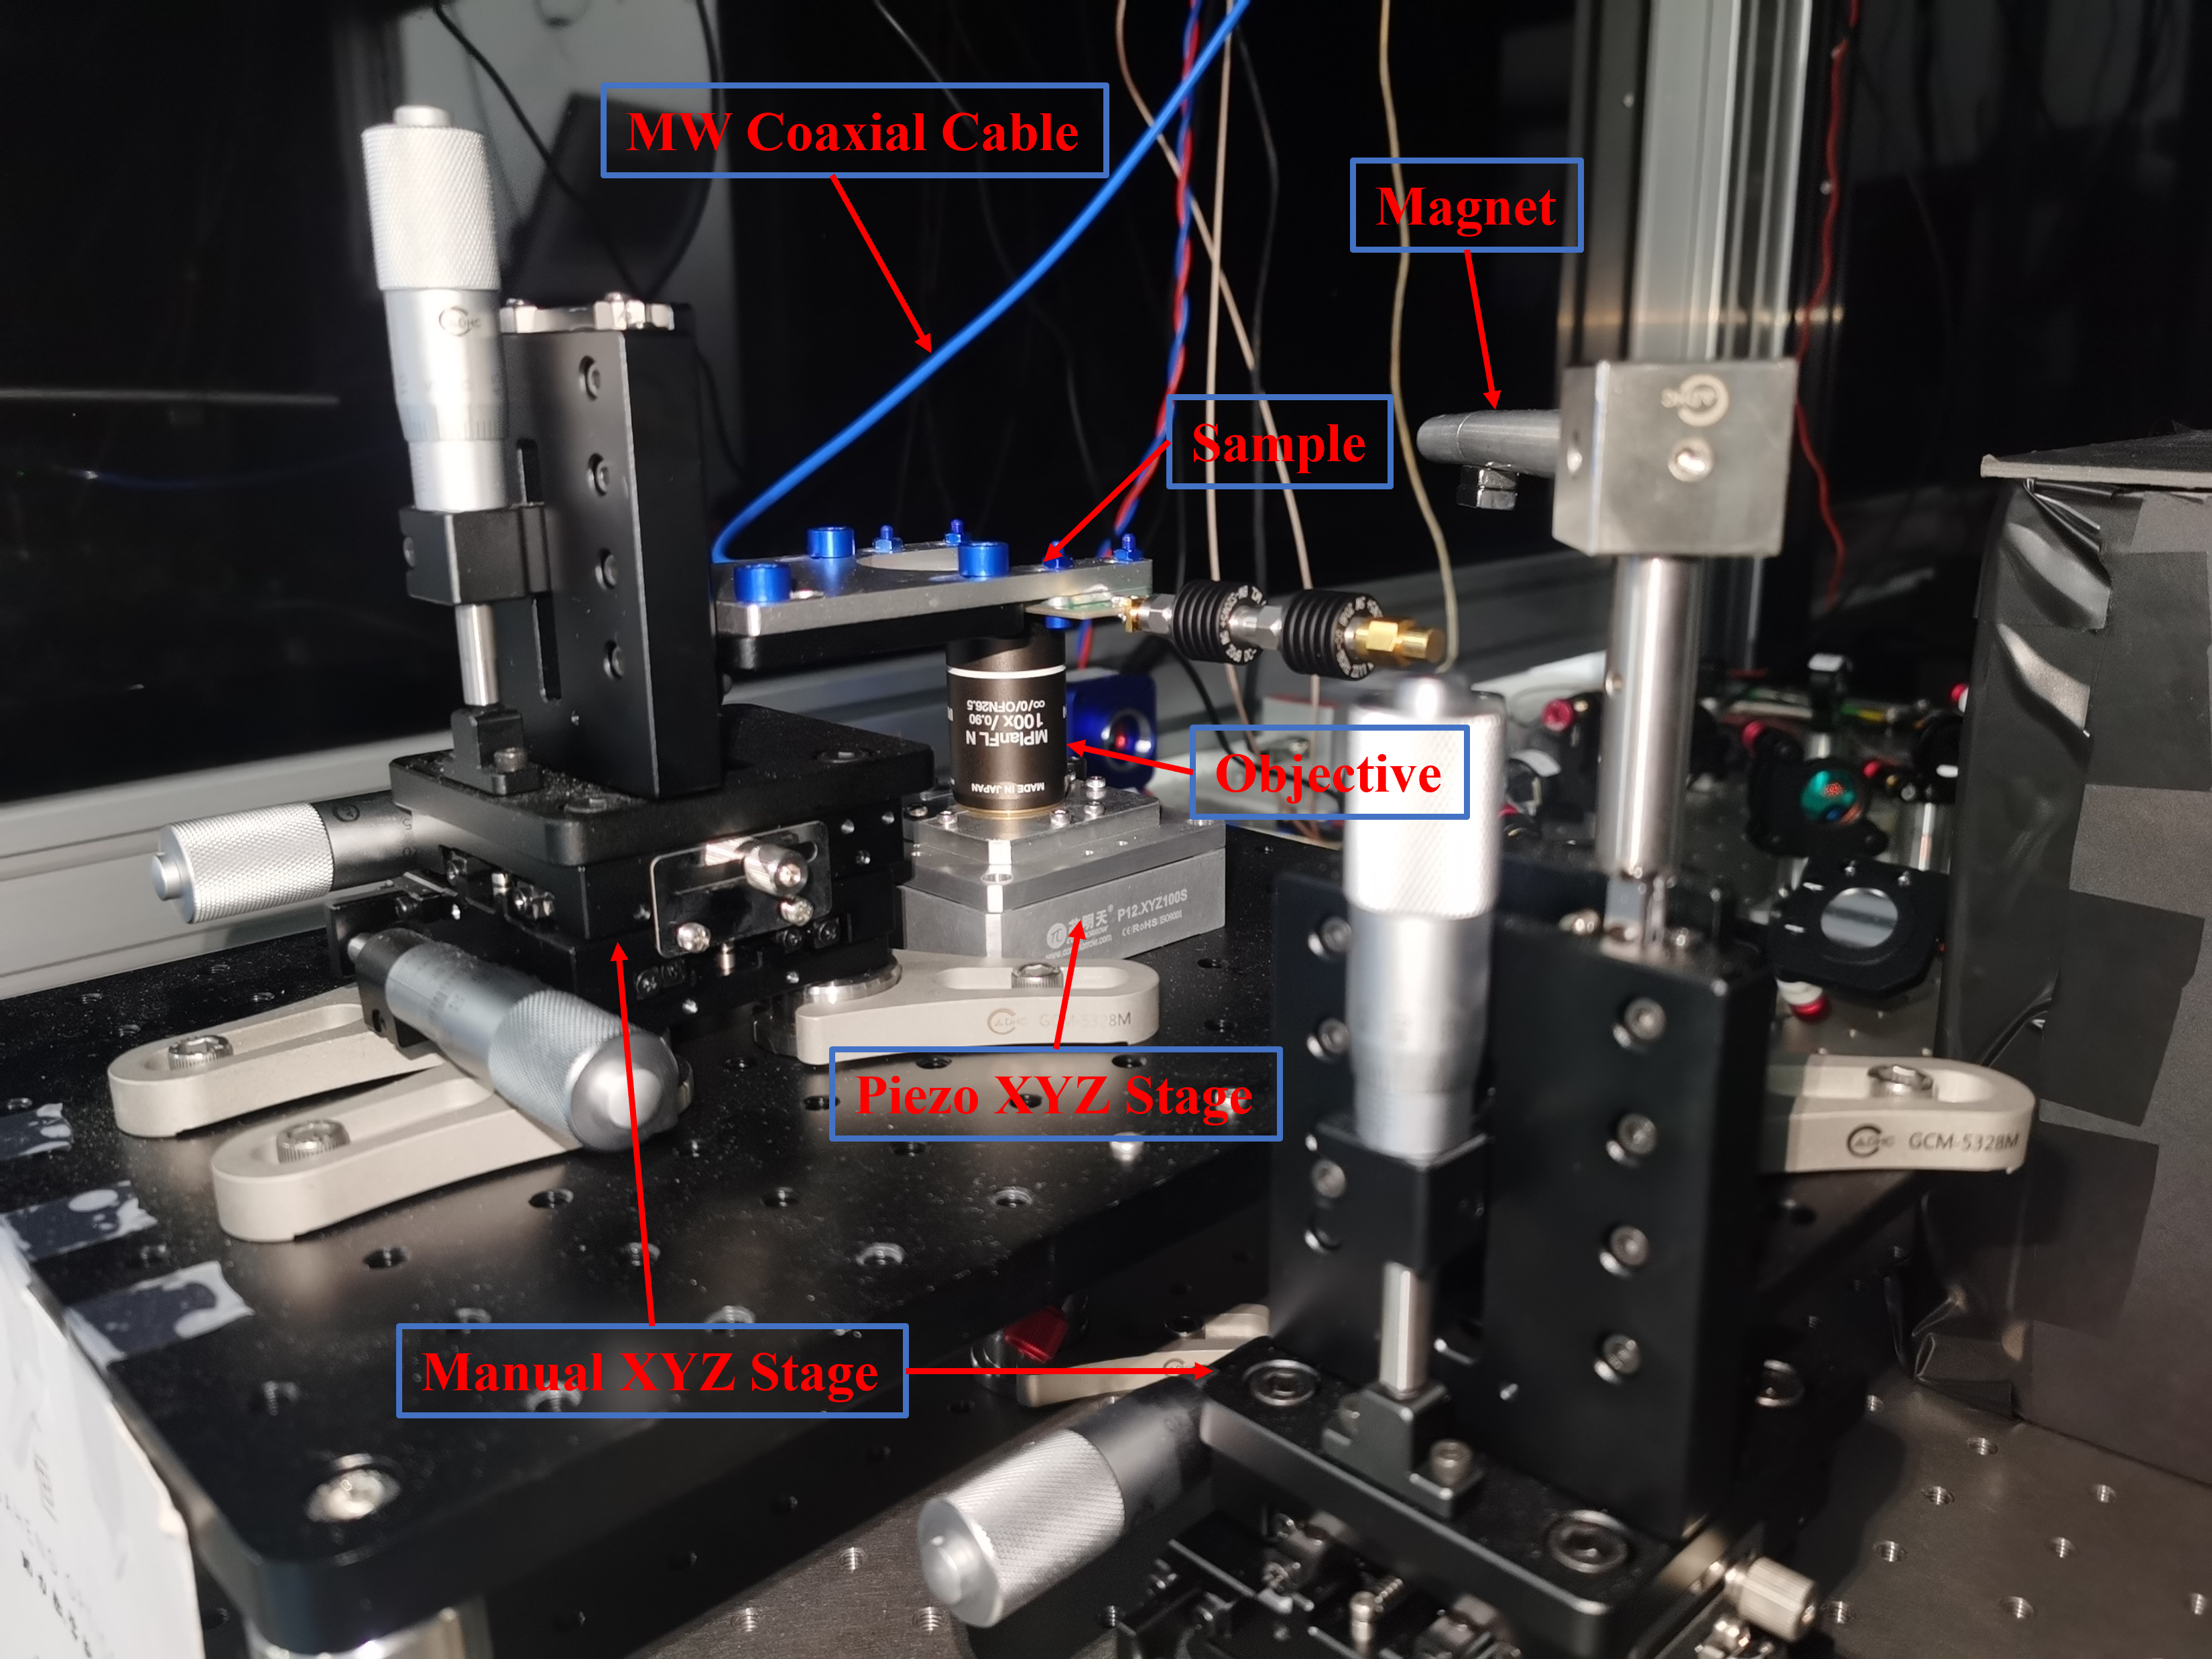
\includegraphics[width=0.8\textwidth]{figures/Chapter 1/Confocal Platform.png}
  \caption[共聚焦显微镜平台]{共聚焦显微镜平台,样品放置于手动XYZ三轴位移台上进行粗调节和聚焦,显微物镜倒置放置于压电纳米XYZ三轴位移台上进行精细扫描和聚焦。微波利用同轴线缆传递到样品表面,磁体也通过三轴手动位移台调节与样品的相对位置。}
  \label{fig: Confocal Platform}
\end{figure}
如图 \ref{fig: Confocal Platform}所示,我们采用的方案是镜头倒置,通过纳米压电位移台移动镜头对样品表面进行扫描的方案。压电位移台为XYZ三轴位移台,移动范围均为100 $\mu m$,精度和稳定性为10 nm的量级,可以实现亚微米级别的扫描和定位。如图 \ref{fig: Confocal Optimizer}所示,展示了Confocal显微镜的Optimize图像,左图为XY方向二维扫描的图像,用于确定NV Center在二维平面的位置;右图为Z方向扫描在不同深度的计数率,用于确定NV Center的深度。我们通过使用的德国Ulm University科研人员开发的基于Python的开源软件Qudi来对整套共聚焦系统进行控制,其中的Optimize功能能够在指定范围内自动寻找计数率高的位置来聚焦寻找NV Center,即图 \ref{fig: Confocal Optimizer}所示效果 \cite{binder2017qudi}。用于测试的样品的NV Center是通过在Element Six公司生产的电子级金刚石表面注入$^{14}$N离子形成的,所以NV Center的位置大部分在离表面5 $\mu m$内的浅层位置,使其发射的荧光光子能够尽可能多的被物镜所接收,提高实验数据和结果的对比度。
\begin{figure}
  \centering
  \includegraphics[width=0.6\textwidth]{figures/Chapter 1/Confocal Optimizer.png}
  \caption[Confocal显微镜的扫描和Auto Optimize功能]{Confocal显微镜的扫描和Auto Optimize功能。}
  \label{fig: Confocal Optimizer}
\end{figure}

\subsection{共聚焦显微镜的搭建}
如图 \ref{fig: Light Path}展示了实验中的光路简图,其中画出了主要元件,一些用于微调调整光路的普通透镜、反射镜、光阑等原件并未画出。对于532 nm的绿光光路而言,激光器产生的激光在出口处耦合进通过光纤输出,光纤用法兰连接光纤声光调制器(Acousto-Optic Modulator,AOM),经过AOM后在通过光纤输出,并在光纤末端用准直器将激光聚焦为高斯光束。AOM是一种通过压电声学效应改变晶体衍射效应,从而对光信号进行调制的器件。我们使用的AOM的驱动器有模拟和数字两个输入口,通过模拟信号输入不同的电压(0-5 V),可以对光强大小进行无级调节;而利用任意波形发生器(Arbitrary Waveform Generator,AWG)产生高频的高低电平,输入给AOM驱动器的数字接口,则可以实现对激光的快速开关,实现特定序列的脉冲测量,其上升沿和下降沿大约为400 ns。激光输出后,通过一个9:1的消偏振分光棱镜(Non-Polarizing Beam Splitter,NPBS),将透射光和反射光的光强分为9:1的两份,且没有改变偏振方向。经过NPBS后,90 \%的透射光透过NPBS继续在光路中传播,而剩下10 \%的反射光则被光电二极管(Photodioad,PD)收集,将光强成比例地转化为电流通过一个定值电阻,通过测量其两端的电压来实时监测光强的大小。经过NPBS的透射光继续传播,穿过550 nm和600 nm截止波长的两个低通二项色镜(Low Pass Dichroic Mirror,LP DM),通过压电位移台设计的孔洞中进入物镜,聚焦于样品表面。前文中有提到过NV Center会受到532 nm的绿光激发后,退激发的过程中发出637 nm的ZPL和波长更长的PSB,这些荧光被同一个物镜收集并原路返回,这些荧光在遇到600 nm LP DM后被反射向左,经过一个663-800 nm的带通滤波片(Band Pass Filter,BP Filter)后,大部分PSB进入单光子雪崩二极管(Avalanche Photodiode,APD)收集,每次收集到一个光子后就会形成脉冲信号,并将数字信号传递给电脑。
\begin{figure}
  \centering
  \includegraphics[width=1.0\textwidth]{figures/Chapter 1/Light Path.png}
  \caption[共聚焦显微镜光路简图]{共聚焦显微镜光路简图。}
  \label{fig: Light Path}
\end{figure}

对于594 nm的橙光光路而言,大部分的设计与532 nm的绿光光路相似,有一点不同的是这个光路中应用的AOM是空间AOM,激光以空间光的形式,通过一个透镜聚焦进入AOM,在出口处相同位置处放置一个相同焦距的透镜来将光束准直。激光经过空间AOM后,会形成多级衍射光斑,其中一级和负一级衍射光斑是可以通过控制AOM来进行调制的,因此我们利用光阑过滤掉了其他光斑,仅留下了一级衍射光斑在光路中继续传播。由于高斯光束在经过AOM后的形状会变得畸形,所以通过物镜耦合进入光纤传递来进行整形,再通过物镜和五维光纤调整架进行准直。如图 \ref{fig: 594 Collimator}所示,通过调整光纤头的位置,对准物镜的出口,准直的高斯光束会从物镜入口处反向射出。由于594 nm的橙光和532 nm的波长不同,导致相差的微小差异,这套装置实际上相当一个可调焦距的准直镜头,将两束激光聚焦于同一平面内。随后,594 nm的橙光通过550 nm LP DM和532 nm的绿光耦合到一起共轴共线,进入显微物镜从而聚焦于样品表面。
\begin{figure}
  \centering
  \includegraphics[width=1.0\textwidth]{figures/Chapter 1/594 Collimator.jpg}
  \caption[594 nm光纤光束准直]{594 nm光纤光束准直,通过物镜和五维光纤调整架对激光进行准直。}
  \label{fig: 594 Collimator}
\end{figure}

\subsection{金刚石样品}
如图 \ref{fig: Sample}所示,样品被粘在铝合金转接板上,转接板和电路板通过蓝色的铝合金螺丝固定,放置铁磁性材料的磁场干扰,或者再施加磁场的过程中受力而发生位移。电路板两头为SMA射频连接头,一头连接混频器发射的微波信号,另一头连接50 $\Omega$的阻抗衰减。中间贯穿的条带为导线,两侧铺铜接地隔离将电磁场束缚在中心,中间部分焊接一根50 $\mu m$粗的铜线作为微波天线,紧贴样品表面使微波在样品表面辐射。微波源(Microwave Source,MW Source)的信号经过放大器,通过混频器(Mixer)和AWG的信号混合后,通向样品电路板的SMA射频连接头。混合AWG信号的目的是在原有设置的恒定的GHz量级的微波信号基础上,加上一个MHz量级的射频信号,从而实现更精细的Pulsed ODMR测量。图中在混频器后省略了微波开关,其功能是通过AWG控制微波的通断来进行特定的序列测量,比如FID、Rabi Oscillation、Hahn-echo Sequence等。
\begin{figure}
  \centering
  \includegraphics[width=1.0\textwidth]{figures/Chapter 1/Sample.jpg}
  \caption[金刚石样品和微波天线结构]{金刚石样品和微波天线结构。}
  \label{fig: Sample}
\end{figure}

\section{测量过程的设计}
\subsection{数据的采集过程}
在测量的过程中,我们选取了两个序列,分别为连续波序列(Continuous Wave,CW)和脉冲序列(Pulsed)两种形式,CW Measurement的目的是为了检测NV Center的电荷态动态平衡分布情况,而Pulsed Measurement的目的是为了将调控电荷的分布并且将自选转化为电荷态进行表征。在整个过程中,我们需要记录的数据只有时间尺度下的荧光发射光子数。在这个过程中,我们利用了时间标记器(Time Tagger,TT),也就是一种基于Opal Kelly FPGA板卡编程设计和开发的时间数字转换器(Time-to-Digital Converter,TDC),可以记录ns级分辨精度的数字信号数据,用于将左右设备的时序逻辑同步对应。我们将AWG和APD的输出都接入到TT上,通过AWG输出序列来控制TT的计数器触发和记录序列,TT接收到高电平的触发信号后,在设定的记录序列接口处于高电平状态的时候就会持续记录数据。与此同时,将AWG连接控制532 nm绿光和594 nm的橙光AOM驱动器,以及微波开关,由此可以通过AWG控制生成的序列来控制激光快速精准的通断和微波的脉冲。这样我们就可以通过控制AWG的输出信号来实现对NV Center的操控和测量。

在准备阶段,我们可以在启动TT的时候设置每一轮测量的最小时间分辨率和整体的时间尺度,以及与物理接口所对应的信号收集通道、触发接口通道和测量脉冲序列通道。在后续的测量过程中,我们设置的最小时间尺度时间窗口(time bins)的分辨率为10 $\mu s$,每一轮测试为10$^6$个time bins,也就是每一轮序列测试是可以持续采集10 $s$的数据,并将原始数据输出为.npy格式的数组保存。在整个测量过程中,我们需要保证样品表面的温度和湿度保持稳定,以及尽可能的减少外部的振动和磁场干扰,以保证测量的准确性和稳定性。由于受到环境变化的干扰,比如温度、湿度、振动等,已经聚焦好的点位会有轻微的漂移现象,所以我们在会对该点进行定时的重新Optimize。我们设置180轮序列测试为一个循环,在一个循环后序列会自动停止,然后click一次Optimize,重新寻找最佳的聚焦点位,然后再次开始下一个循环,并将所有的180个数据保存到本地文件中。通过设置不同的循环次数,我们能够定制不同的数据累积时间,从而保证不同情况下数据量尽可能地归一性。


\subsection{测量序列的设置和数据的处理}

如图 \ref{fig: Measurement Sequence}所示,(a)图为CW测量序列,(b)图为Pulsed测量序列。
\begin{figure}
  \centering
  \includegraphics[width=1.0\textwidth]{figures/Chapter 1/Measurement Sequence.png}
  \caption[CW和Pulsed测量序列简图]{CW和Pulsed测量序列简图,$t_r$为读出时间窗口,$t_{ini}$为初始化时间长度。}
  \label{fig: Measurement Sequence}
\end{figure}

对于(a)图中CW序列而言,在每一轮10 $s$的测试过程中,594 nm的橙光持续保持开启的状态。由于AOM的开启存在上升沿和稳定性的问题,每次TT计数器的触发接口在开启橙光后10 $\mu s$后,施加一个50 $ns$的高电平脉冲,使计数器启动。随后TT计数器的测量脉冲序列通道保持10 $s$的高电平状态,在这个过程中,TT以10 $\mu s$为时间分辨率窗口进行持续地记录数据。序列结束的时候,保持橙光持续开启2 $\mu s$,以确保测量序列末端的光强稳定。因为是连续测量,所以在设置不同的读出时间$t_r$的时候,只需要间隔不同数量的相邻time bins进行合并,即可得到不同的$t_r$,即$t_r = n_{merge} \times 10\ \mu s$,然后将结果归一化,利用$Python$中的$Matplotlib$包绘制以对数坐标为纵轴概率,以每个$t_r$内的光子数为横轴事件的概率分布直方图。

对于(b)图中的Pulsed序列而言,每次用532 nm的绿光初始化序列长度为$t_{ini} = 3\ \mu s$,随后有一段长为$t_{wait} = 1\ \mu s$的间隔,使电荷态充分转换并稳定,最后是利用 594 nm的橙光进行读出,TT计数器也同时启动,记录APD接受光子生成的脉冲序列。数据后处理和绘图的方式和CW序列相同。

在数据拟合的过程中,我们应用了$SciPy$中的“$curve\_fit$”函数,根据第二章中的理论模型,拟合出最合适的参数,并确定拟合的标准差(Standard Deviation,STD)。同时通过改变$n_{merge}$的值来改变$t_r$,使得最后的STD尽可能的小。$t_r$过大的时候,大量的time bins合并在一起,使数据的密度过大,从而难以得到合理的分布规律;而较小的$t_r$会使得数据的密度过小,可能出现的情况较少,可用于拟合的数据点不足,难以得到合理的拟合结果。

 
\end{document}